\documentclass[english]{maciarticle}

\usepackage{amsmath,amsbsy,amscd,amssymb,graphicx, epsfig,color,float,cite}

%%%%%%%%%%%%%%%%%%%%%%%%%%%%%%%%%%%%%%%%%%%%%
\begin{document}

\title{Hierarchical Risk Parity for Cryptocurrency Portfolios: A Comparative Analysis}

\author[$\flat$]{Alan Matys}
\author[$\flat$]{Federico Martin Rodriguez}
\affil[$\flat$]{Universidad del CEMA,
\textcolor{blue} {alan.matys92@gmail.com, federico.m.rodriguez.h@gmail.com}}

\maketitle

\begin{abstract}
This article addresses portfolio construction as a budget allocation problem, balancing expected returns with risk mitigation. Traditional methods like the Critical Line Algorithm (CLA) struggle with diversification due to their sensitivity to input parameters. Hierarchical Risk Parity (HRP) offers a robust alternative by employing correlation-based clustering and hierarchical weight allocation. We evaluate HRP’s effectiveness in cryptocurrency markets, where traditional optimization methods face challenges due to high volatility and inter-asset correlations. Our findings demonstrate that HRP achieves superior diversification while maintaining computational stability, making it a compelling choice for risk-based asset allocation.
\end{abstract}

\begin{keywords}
Hierarchical Risk Parity, Risk-based asset allocation, Cryptocurrency, Portfolio Optimization
\end{keywords}

\begin{mathsubclass}
21A54 - 55P54
\end{mathsubclass}

{\thispagestyle{empty}} %DO NOT DELETE THIS LINE

%%===============================
\section{Introduction}
%%===============================

The portfolio construction problem is central to finance, requiring investors to strategically allocate capital to balance risk and return \cite{markowitz1952}. Traditional mean-variance optimization techniques, such as the Markowitz Critical Line Algorithm (CLA), are widely used but are highly sensitive to input estimates, often leading to unstable and concentrated allocations \cite{lopez2016}. Additionally, these methods rely on inverting the variance-covariance matrix, which can introduce numerical instability when dealing with large or ill-conditioned datasets.

To address these limitations, \textbf{Hierarchical Risk Parity (HRP)} has been proposed as an alternative, leveraging hierarchical clustering to construct diversified portfolios without requiring matrix inversion \cite{lopez2016}. HRP has demonstrated improved robustness in asset allocation, particularly in scenarios with unstable correlation structures and high-dimensional datasets \cite{lopez2018}. This study applies HRP to cryptocurrency markets, evaluating its effectiveness in achieving portfolio diversification compared to traditional optimization methods.

%%===============================
\section{HRP Portfolio Building}
%%===============================

The HRP algorithm consists of three key steps: hierarchical clustering, quasi-diagonalization, and recursive bisection. Unlike traditional mean-variance optimization, HRP does not require matrix inversion, making it particularly robust when dealing with unstable correlation structures or singular covariance matrices \cite{lopez2018}. The methodology leverages clustering techniques to group correlated assets, reorganizes the covariance matrix for improved numerical stability, and recursively assigns weights to construct a risk-balanced portfolio.

\subsection{Hierarchical Clustering}

HRP begins by clustering assets based on their correlation structure. The correlation matrix is defined as:
\[
\rho = \left( \rho_{i,j} \right)_{i,j=1,...,N}
\]
where each element \(\rho_{i,j}\) represents the correlation between asset \(X_i\) and asset \(X_j\):
\[
\rho_{i,j} = \rho[X_i, X_j].
\]
Since correlation values are bounded within \([-1,1]\), their absolute scale does not impact the clustering process. To measure dissimilarity between assets, a distance metric is introduced:
\[
d : (X_i, X_j) \subseteq \mathcal{B} \to \mathbb{R} \in [0, 1], \quad d_{i,j} = d[X_i, X_j] = \sqrt{\frac{1}{2}(1 - \rho_{i,j})}.
\]
where \(\mathcal{B}\) represents the Cartesian product of asset pairs. Using this distance matrix, hierarchical clustering is performed by computing Euclidean distances between matrix columns:
\[
\tilde{d} : (D_i, D_j) \subseteq \mathcal{B} \to \mathbb{R} \in [0, \sqrt{N}], \quad \tilde{d}_{i,j} = \tilde{d}[D_i, D_j] = \sqrt{\sum_{n=1}^N (d_{n,i} - d_{n,j})^2}.
\]
A linkage criterion is then applied to merge clusters recursively, forming a tree-based structure that groups assets with similar risk characteristics.

\subsection{Quasi-Diagonalization}

Once hierarchical clustering is completed, the covariance matrix is reordered to improve numerical stability. The linkage matrix from the clustering process provides an ordering that is used to rearrange the covariance matrix. This transformation is represented as:
\[
\tilde{\Sigma} = P \Sigma P^T
\]
where \( P \) is the permutation matrix derived from the clustering structure. The reordering ensures that correlated assets are placed adjacent to each other, while uncorrelated or negatively correlated assets are positioned farther apart. As a result, large values in the covariance matrix align along the diagonal, preserving the hierarchical clustering structure and enhancing the stability of subsequent computations.

\subsection{Recursive Bisection for Portfolio Allocation}

The final stage of HRP is the recursive bisection process, which assigns portfolio weights while maintaining risk balance. The algorithm proceeds as follows:

\textbf{Step 1 (Initialization):}
Define the full asset set \(L_0 = \{ n \}_{n=1,...,N}\) and assign equal initial weights \(w_n = 1, \quad \forall n = 1, ..., N\).

\textbf{Step 2 (Recursive Weight Allocation):}
For each subset \( L_i \), if \( |L_i| = 1 \), the final weight is assigned to the asset. Otherwise, split \( L_i \) into two subgroups \( L_a \) and \( L_b \) using hierarchical clustering. The risk contribution of each subgroup is then computed using inverse variance allocation:
\[
w_a = \frac{1 / \sum_{i \in L_a} \sigma_i}{1 / \sum_{i \in L_a} \sigma_i + 1 / \sum_{j \in L_b} \sigma_j}
\]
\[
w_b = 1 - w_a
\]
where \( \sigma_i \) represents the standard deviation of asset \( i \). This bisection process is recursively applied to each subgroup until all assets are individually assigned weights.

\subsection{Final Portfolio Composition}

The final portfolio weights obtained from HRP maintains diversification by clustering correlated assets together, enhances numerical stability through covariance matrix quasi-diagonalization, and achieves a risk-balanced allocation without requiring matrix inversion.

Empirical studies show that HRP produces lower out-of-sample variance than traditional mean-variance approaches, making it a robust choice for asset allocation in complex financial markets \cite{lopez2018}.

%%===============================
\section{Results and Evaluation Methodology}
%%===============================

The proposed method is tested against traditional portfolio allocation techniques, including the Inverse Variance Portfolio (IVP) and the Minimum Variance Portfolio (MVP), as well as against holding BTC and ETH for the entire backtesting period. The backtesting period spans from \textbf{January 1, 2021, to January 1, 2024}. For the construction of the portfolio, we consider assets with at least two years of trading history. Additionally, pairs involving dollar stablecoins are filtered out to ensure the focus remains on assets with significant market activity and volatility.

The methodology is assessed under two distinct scenarios: static portfolio allocation, where weights are assigned once at the beginning of the backtesting period without rebalancing, and monthly rebalancing, where the best-performing method from the static scenario is compared with the three methodologies under a monthly rebalancing strategy with market data from Binance, incorporating a transaction cost rate of 0.1\% per trade as referenced from Binance's basic trading fee.

\subsection{Evaluation Metrics}

Portfolio performance is assessed using key financial metrics widely adopted in investment analysis. \textbf{Total Return (\%)} quantifies the cumulative percentage change in portfolio value over time \cite{bacon2008}. \textbf{Annualized Volatility (\%)} measures return dispersion, reflecting overall risk exposure \cite{markowitz1952}. \textbf{Sharpe Ratio} evaluates excess returns per unit of total risk \cite{sharpe1994}, while the \textbf{Sortino Ratio} refines this by focusing on downside deviations \cite{sortino1994}. \textbf{Maximum Drawdown (\%)} captures the largest decline from peak to trough, crucial for risk management \cite{young1991}. The \textbf{Calmar Ratio} extends this by assessing return efficiency relative to drawdown \cite{young1991}. These metrics, used extensively in portfolio construction and risk assessment \cite{lopez2016, lopez2018}, provide a comprehensive view of performance under different market conditions.

By integrating these risk and return measures, investors can compare portfolio efficiency, evaluate stability, and optimize asset allocation strategies for improved long-term results \cite{demiguel2009}.

%%===============================
\subsection{Results}
%%===============================

The results for static portfolio allocation are presented in Figure 1 and Table 1. The MVP method demonstrates superior diversification and risk-adjusted returns compared to other methods.

\begin{figure}[H]
    \centering
    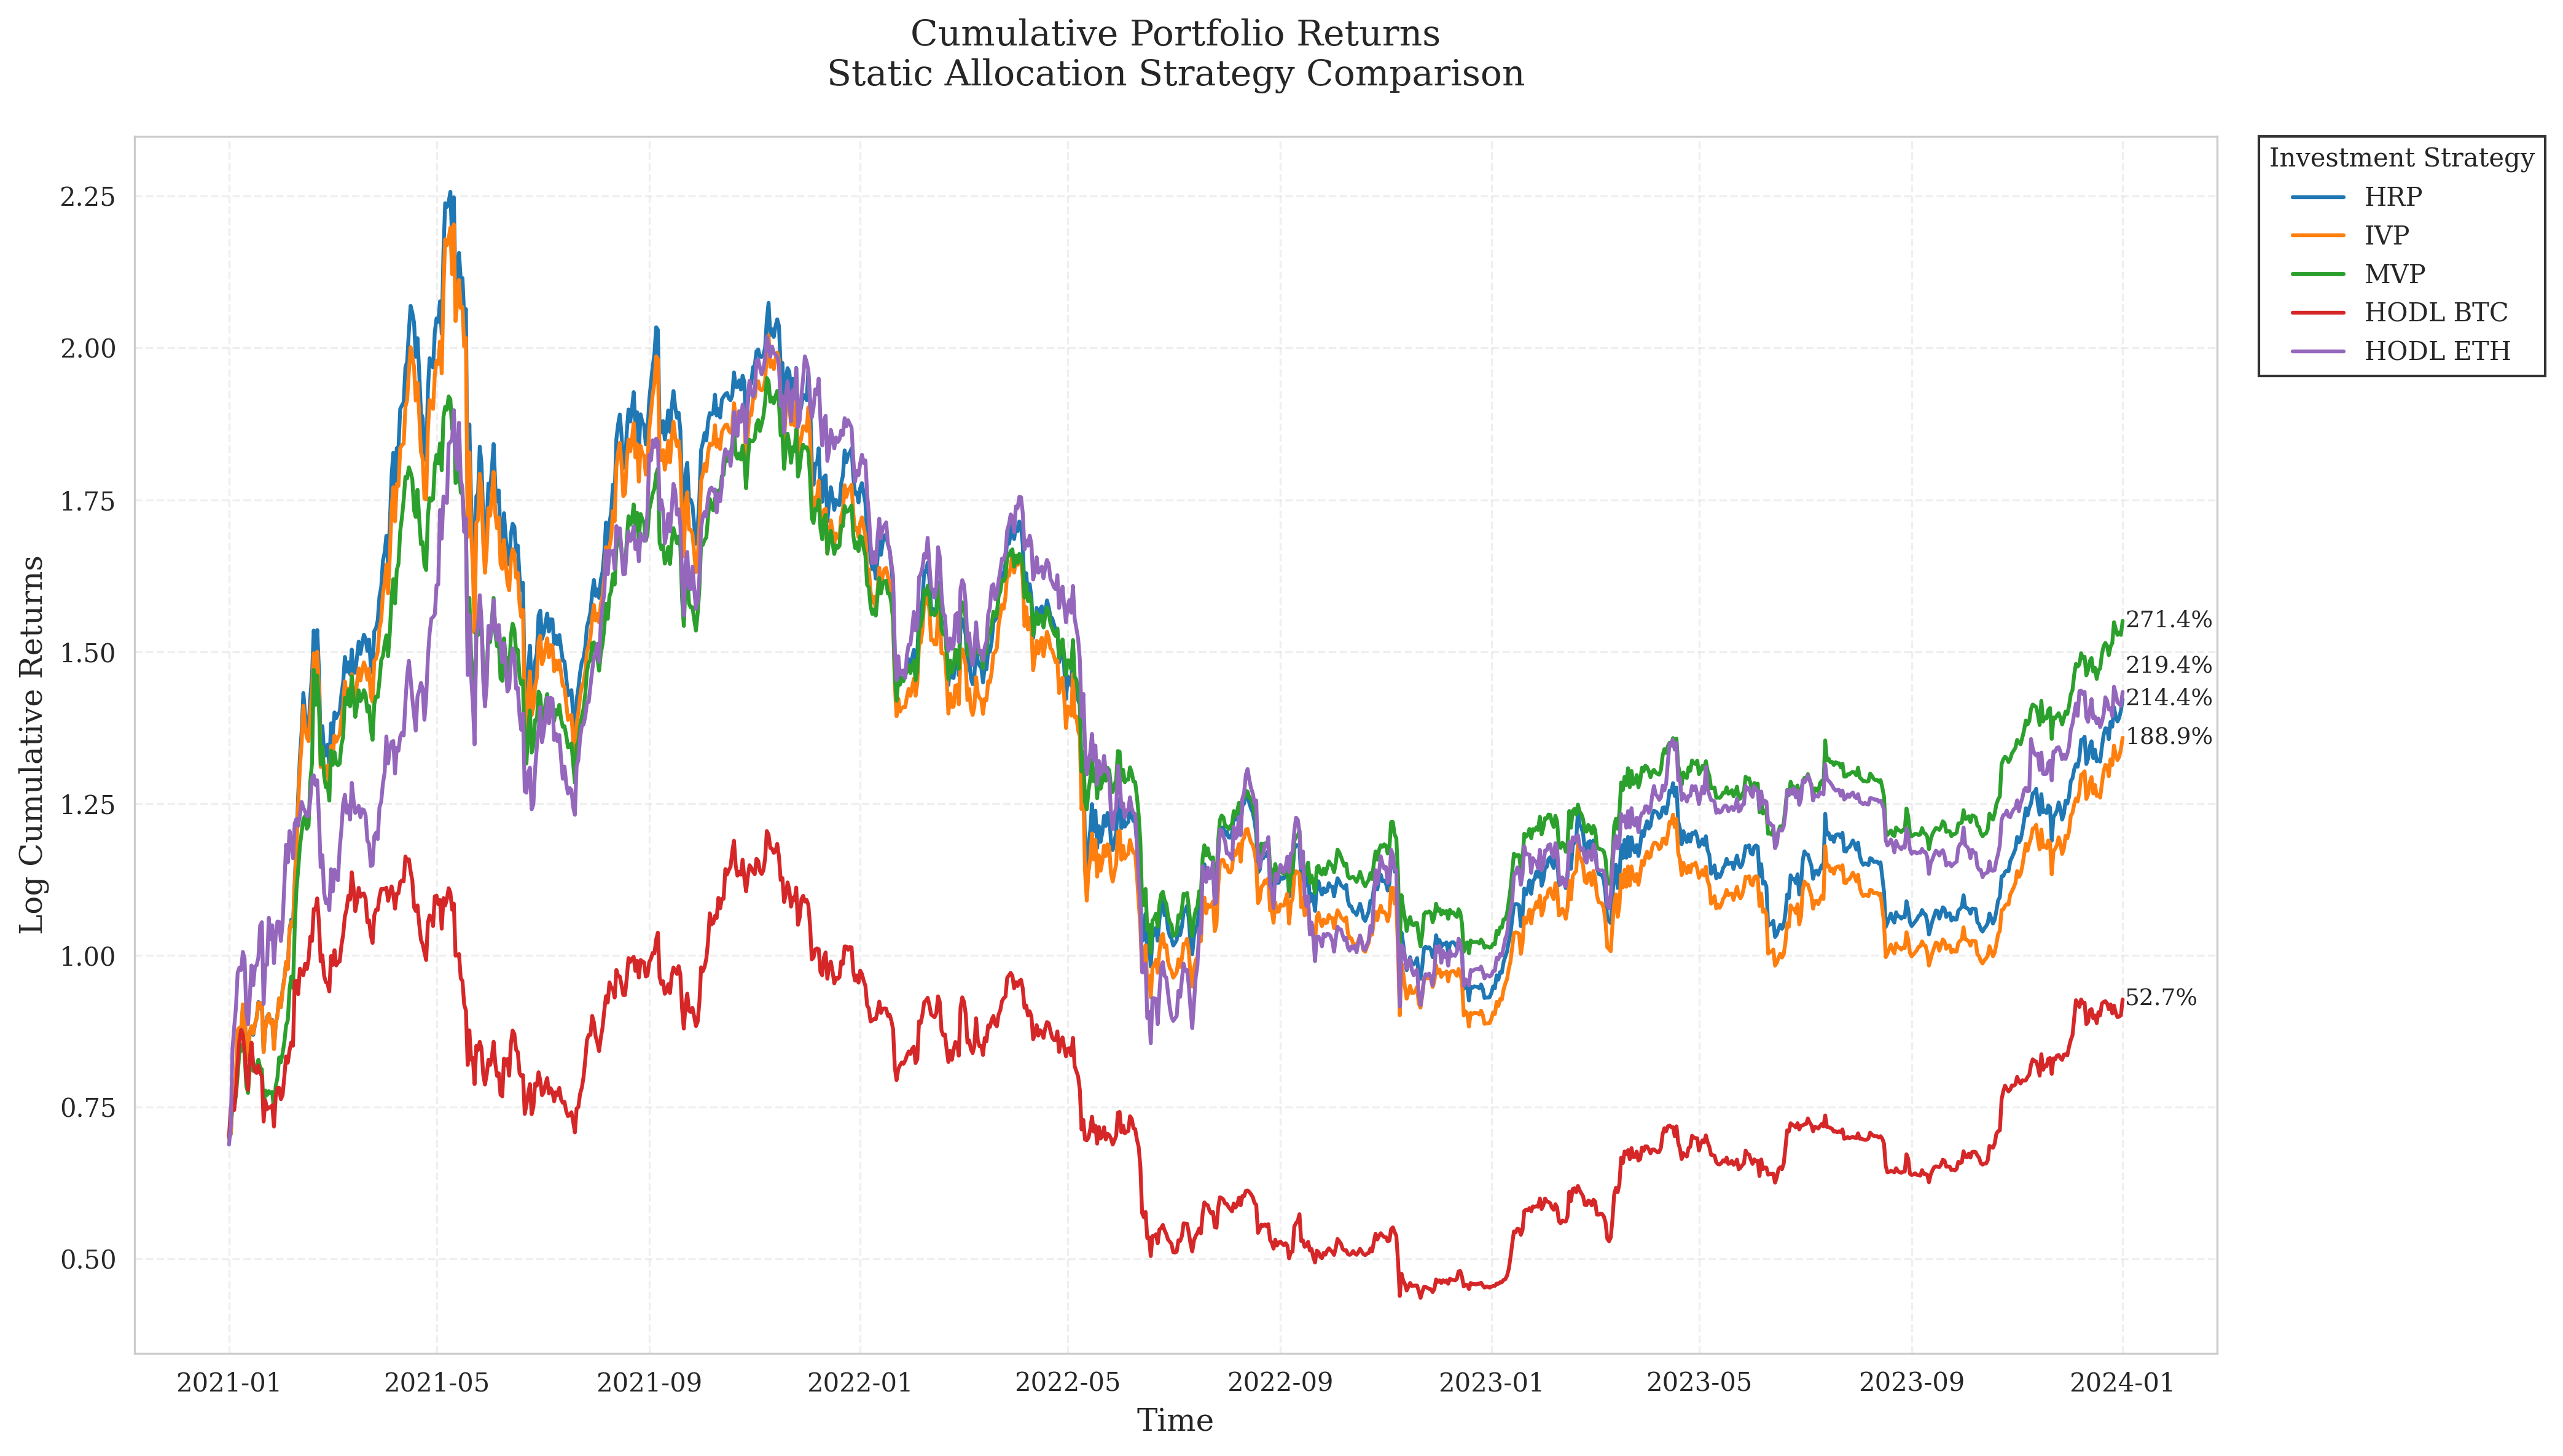
\includegraphics[width=0.8\textwidth]{static_cumulative_returns.png}
    \caption{Cumulative Returns for Static Portfolio Allocation.}
    \label{fig:static_cum_returns}
\end{figure}

\vspace{-0.5cm}

\begin{table}[H]
    \centering
    \renewcommand{\arraystretch}{1.1}
    \small % Reduce font size
    \caption{Performance Metrics for Static Portfolio Allocation}
    \begin{tabular}{|l|c|c|c|c|c|c|}
    \hline
    Portfolio & Total Return (\%) & Ann. Volatility (\%) & Sharpe Ratio & Sortino Ratio & Max Drawdown (\%) & Calmar Ratio \\
    \hline
    HRP & 214.45 & 82.17 & 0.88 & 0.82 & -82.21 & 0.57 \\
    IVP & 188.86 & 82.07 & 0.85 & 0.79 & -82.42 & 0.51 \\
    MVP & 271.45 & 70.51 & 0.97 & 0.98 & -71.38 & 0.77 \\
    HODL BTC & 52.75 & 64.86 & 0.54 & 0.57 & -76.63 & 0.20 \\
    HODL ETH & 219.39 & 84.68 & 0.88 & 0.91 & -79.30 & 0.60 \\
    \hline
    \end{tabular}
\end{table}

In the monthly rebalancing scenario, shown in Figure 2 and Table 2, HRP and IVP outperform, highlighting their robustness in dynamic market conditions.

\begin{figure}[H]
    \centering
    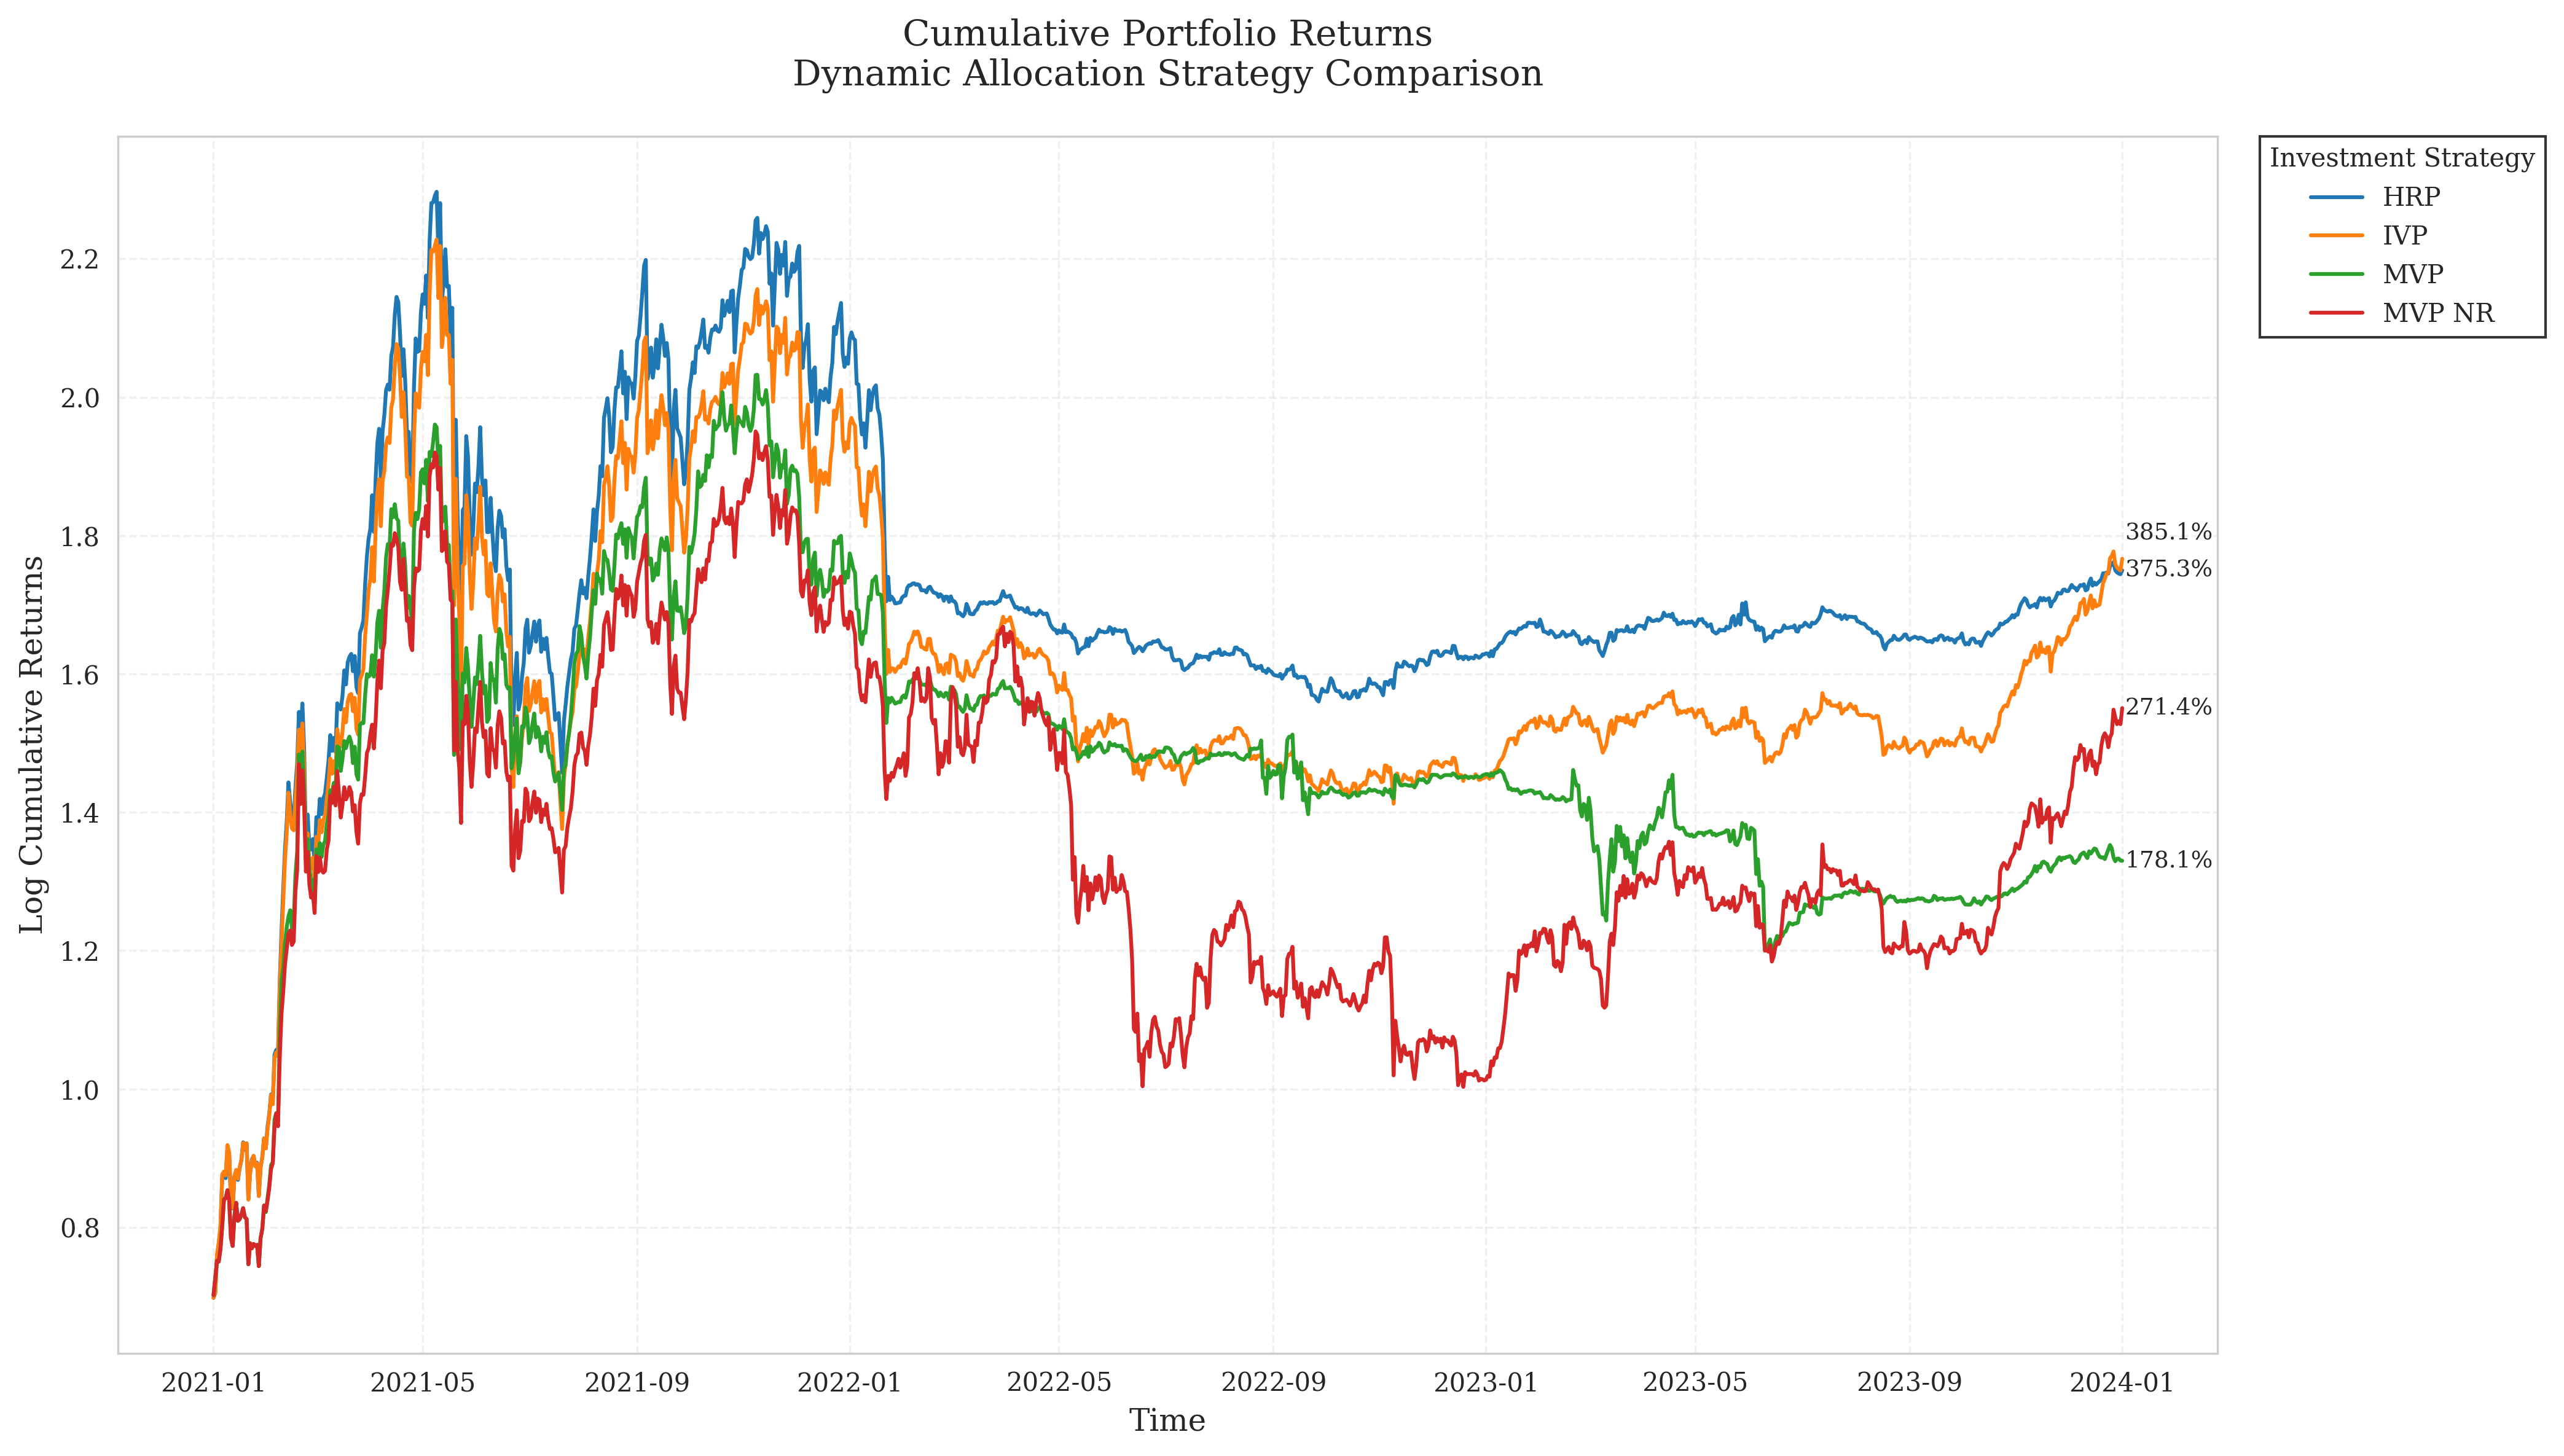
\includegraphics[width=0.8\textwidth]{rebalancing_cumulative_returns.png}
    \caption{Cumulative Returns for Monthly Rebalancing.}
    \label{fig:rebalance_cum_returns}
\end{figure}

\vspace{-0.5cm}

\begin{table}[H]
    \centering
    \renewcommand{\arraystretch}{1.1}
    \small % Reduce font size
    \caption{Performance Metrics for Monthly Rebalancing}
    \begin{tabular}{|l|c|c|c|c|c|c|}
    \hline
    Portfolio & Total Return (\%) & Ann. Volatility (\%) & Sharpe Ratio & Sortino Ratio & Max Drawdown (\%) & Calmar Ratio \\
    \hline
    MVP NR & 271.45 & 70.51 & 0.97 & 0.98 & -71.38 & 0.77 \\
    HRP & 375.32 & 68.41 & 1.11 & 1.09 & -63.17 & 1.08 \\
    IVP & 385.06 & 68.92 & 1.12 & 1.06 & -64.28 & 1.08 \\
    MVP & 178.09 & 60.87 & 0.87 & 0.90 & -65.31 & 0.62 \\
    \hline
    \end{tabular}
\end{table}

%%===============================
\section{Conclusion \& Future Research}
%%===============================

In conclusion, for static portfolios, the MVP exhibits superior diversification and risk-adjusted returns. However, with monthly rebalancing, HRP and IVP outperform, showcasing their adaptability to dynamic market conditions. The observed concentration in rebalanced portfolios and the sensitivity of MVP strategies to rebalancing costs highlight the importance of considering transaction costs in portfolio management.

Future research should focus on refining HRP to address noise from small eigenvalues in the correlation matrix and to account for market-wide correlation shocks by filtering out systemic movements. Additionally, exploring alternative distance metrics and clustering techniques within the HRP framework could further enhance its performance.

%%===============================
\section*{Acknowledgements}
%%===============================

We thank the UCEMA Quant faculty, particularly Manuel Maurette, Emiliano Delfau and Pablo Martin Gechidjian, as well as Marcos López de Prado for his seminal contributions to the field.

\begin{thebibliography}{9}

\bibitem{markowitz1952} 
Markowitz, H. (1952). \textit{Portfolio Selection}. The Journal of Finance, 7(1), 77-91.

\bibitem{lopez2016}
López de Prado, M. (2016). \textit{Building Diversified Portfolios that Outperform Out-of-Sample}. Journal of Portfolio Management.

\bibitem{lopez2018}
López de Prado, M. (2018). \textit{Advances in Financial Machine Learning}. John Wiley \& Sons.

\bibitem{lopez2020} 
López de Prado, M. (2020). \textit{Machine Learning for Asset Managers}. Cambridge University Press.

\bibitem{bacon2008} 
Bacon, C. (2008). \textit{Practical Portfolio Performance Measurement and Attribution}. John Wiley \& Sons.

\bibitem{sharpe1994} 
Sharpe, W. F. (1994). \textit{The Sharpe Ratio}. Journal of Portfolio Management, 21(1), 49-58.

\bibitem{sortino1994} 
Sortino, F., \& Price, L. (1994). \textit{Performance Measurement in a Downside Risk Framework}. Journal of Investing, 3(3), 59-64.

\bibitem{young1991} 
Young, T. W. (1991). \textit{Calmar Ratio: A Smoother Tool}. Futures Magazine, 20(2), 40-41.

\bibitem{demiguel2009}
De Miguel, V., Garlappi, L., \& Uppal, R. (2009). \textit{Optimal Versus Naive Diversification: How Inefficient is the 1/N Portfolio Strategy?} The Review of Financial Studies, 22(5), 1915-1953.

\end{thebibliography}

\end{document}